%!TEX program = lualatex
\documentclass[aspectratio=169,11pt]{beamer}

\usepackage{draftwatermark}

\usepackage{tikz}
\usetikzlibrary{calc}

\setbeamertemplate{background}{%
  \begin{tikzpicture}[remember picture,overlay]
    \node[
      rotate=45,
      scale=4.5,
      text opacity=0.08
    ] at (current page.center) {RASCUNHO};
  \end{tikzpicture}%
}

% ===== Tema / aparência =====
\usetheme{Madrid}
\usecolortheme{whale}
\setbeamertemplate{navigation symbols}{}

% ===== Idioma =====
\usepackage[portuguese]{babel}

% ===== Fonte (LuaLaTeX) =====
\usepackage{fontspec}
\setmainfont{Latin Modern Roman}

% ===== Figuras / tabelas =====
\usepackage{graphicx}
\usepackage{booktabs}

% ===== Links =====
\usepackage{xurl}
\Urlmuskip=0mu plus 1mu

%=======Lipsum============
\usepackage{lipsum}

% ===== Logo na capa =====
\titlegraphic{
\includegraphics[width=1.8cm]{uerj.jpg}}

% ===== Metadados =====
\title[Seminário de Cartografia X]{Seminário de Cartografia X}
\subtitle{Caracterização fisiográfica e aspectos oceanográficos do litoral de Atafona}
\author[Carneiro, Gaiani e Elsas]{%
Israel de Oliveira Carneiro \and Miguel Gayani \and José Mauro Elsas
}
\institute[UERJ]{Universidade do Estado do Rio de Janeiro \\Faculdade de Oceanografia}
\date{março de 2026}

\begin{document}

% ===== Capa =====
\begin{frame}
  \titlepage
  \section{Objetivo}
  \section{Caracterização Fisiográfica de Atafona}
  \section{Metodologia}
  \section{Discussão e Resultados}
  \section{Referências}
\end{frame}

% ===== Sumário =====
\begin{frame}{Sumário}
  \tableofcontents
\end{frame}

\begin{frame}{Objetivo}
  \lipsum[1]
\end{frame}

\begin{frame}{Caracterização Fisiográfica de Atafona}
\begin{columns}[T,onlytextwidth]
    \begin{column}{0.48\textwidth}
        \textbf{Texto sobre caracterização.}
        \begin{itemize}
            \item Primeiro ponto
            \item Segundo ponto
            \item Terceiro ponto.
        \end{itemize}
    \end{column}

    \begin{column}{0.48\textwidth}
        \centering
        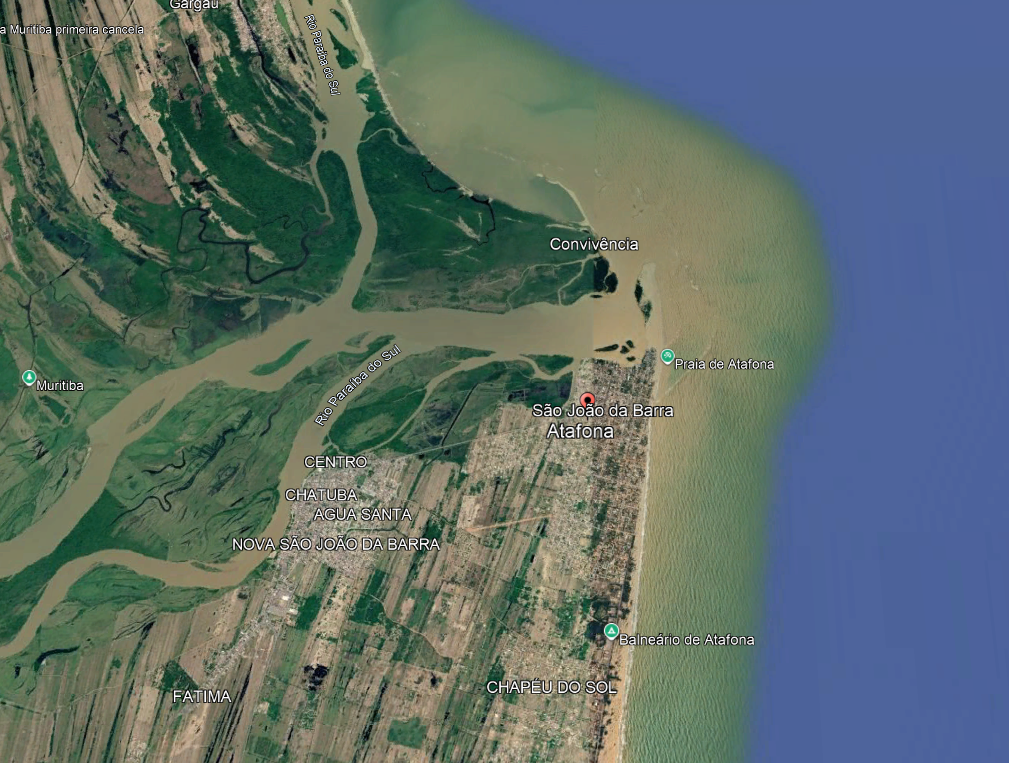
\includegraphics[width=\linewidth]{Atafona_1.png}
        
        \vspace{0.3em}
        {\footnotesize Atafona, São João da Barra}
    \end{column}
\end{columns}
\end{frame}

\begin{frame}{Metodologia}
\begin{columns}[T,onlytextwidth]
    \begin{column}{0.48\textwidth}
        \textbf{Texto sobre a metodologia.}
        \begin{itemize}
            \item Primeiro ponto
            \item Segundo ponto
            \item Terceiro ponto.
        \end{itemize}
    \end{column}

    \begin{column}{0.48\textwidth}
        \centering
        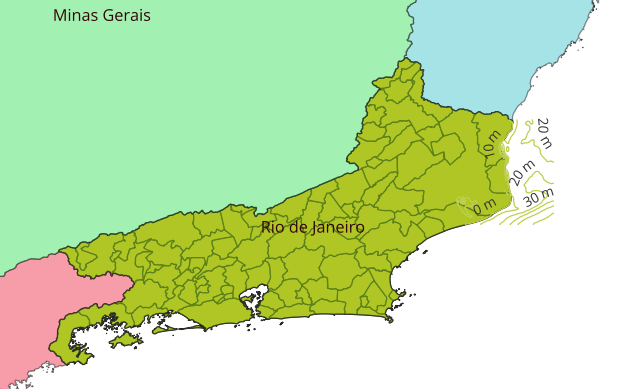
\includegraphics[width=\linewidth]{rj_regiao.png}
        
        \vspace{0.3em}
        {\footnotesize Rio de Janeiro}
    \end{column}
\end{columns}
\end{frame}

\begin{frame}{Discussão e Resultados}
\begin{columns}[T,onlytextwidth]
    \begin{column}{0.48\textwidth}
        \textbf{Texto sobre os resultados.}
        \begin{itemize}
            \item Primeiro ponto
            \item Segundo ponto
            \item Terceiro ponto.
        \end{itemize}
    \end{column}

    \begin{column}{0.48\textwidth}
        \centering
        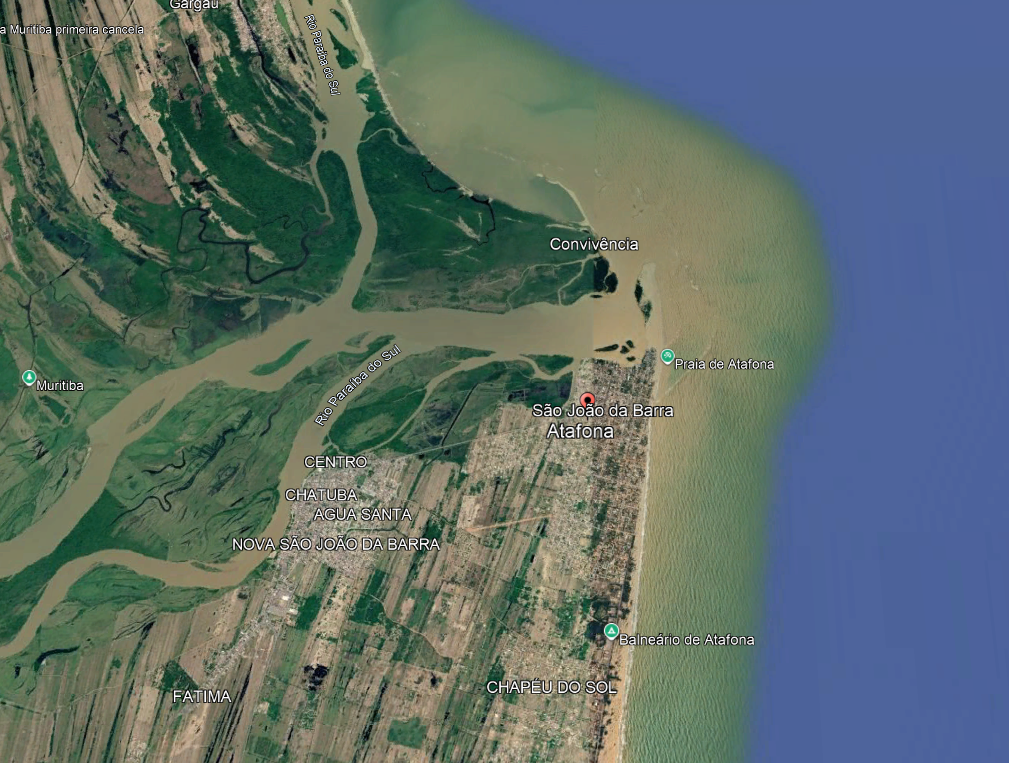
\includegraphics[width=\linewidth]{Atafona_1.png}
        
        \vspace{0.3em}
        {\footnotesize Atafona, São João da Barra}
    \end{column}
\end{columns}
\end{frame}

\begin{frame}{Discussões e Recomendações}
\begin{columns}[T,onlytextwidth]
    \begin{column}{0.48\textwidth}
        \textbf{Texto sobre Discussões e remomencações.}
        \begin{itemize}
            \item Primeiro ponto
            \item Segundo ponto
            \item Terceiro ponto.
        \end{itemize}
    \end{column}

    \begin{column}{0.48\textwidth}
        \centering
        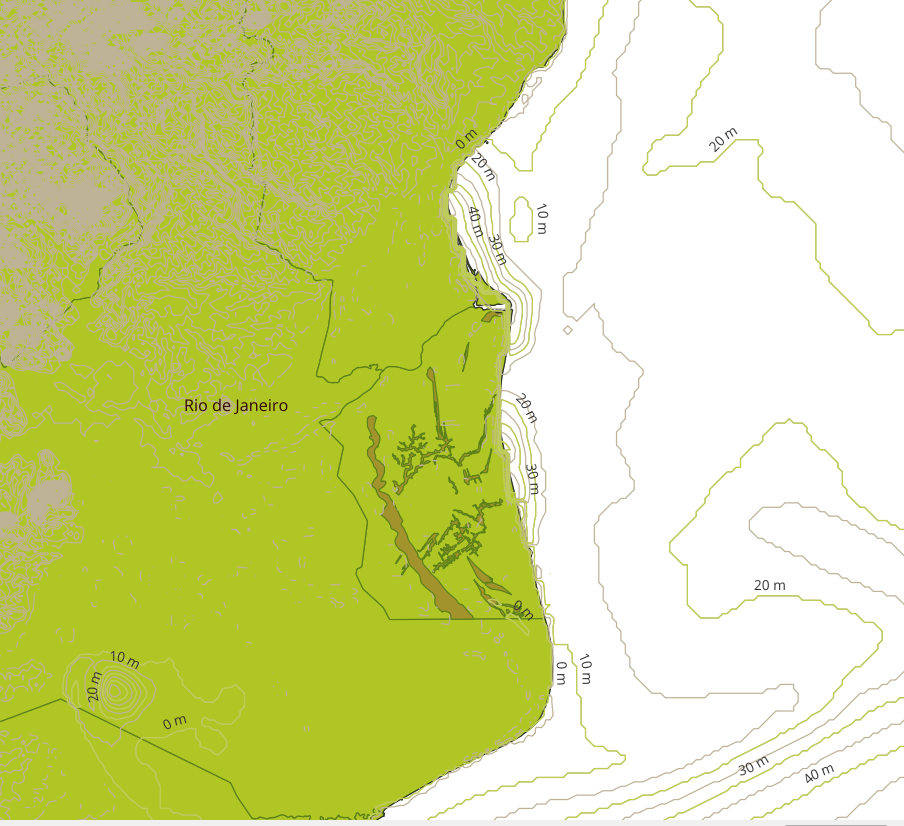
\includegraphics[width=0.5\linewidth]{norte_rj.png}
        
        \vspace{0.3em}
        {\footnotesize Atafona, São João da Barra}
    \end{column}
\end{columns}
\end{frame}

  \begin{frame}{Referências}

  \begin{itemize}
    \item Ref 1
    \item Ref 2
    \item Ref 3
  \end{itemize}
  
\end{frame}

\end{document}